\chapter{Case study}

The case study describes a measuring system deployment on a mechanism that was the motivation for this project. The mechanism shown in figures \ref{fig:mbs} - \ref{fig:render} is an overconstrained multibody system \cite{bib:BPAS2012} that consists of a moving platform connected to the ground by 6 rigid rods. The rods have equal lengths. In the assembly variant shown in the figures, all lower and upper rods, respectively, are parallel to each other. The mechanism has one degree of freedom (plus 6 internal mobilities), except for two points where a bifurcation occurs. Due to this property, it is hard to simplify the mechanism model to a minimal set of coordinates.

\begin{figure}[!h]
	\centering
	\begin{minipage}{.5\textwidth}
		\centering
		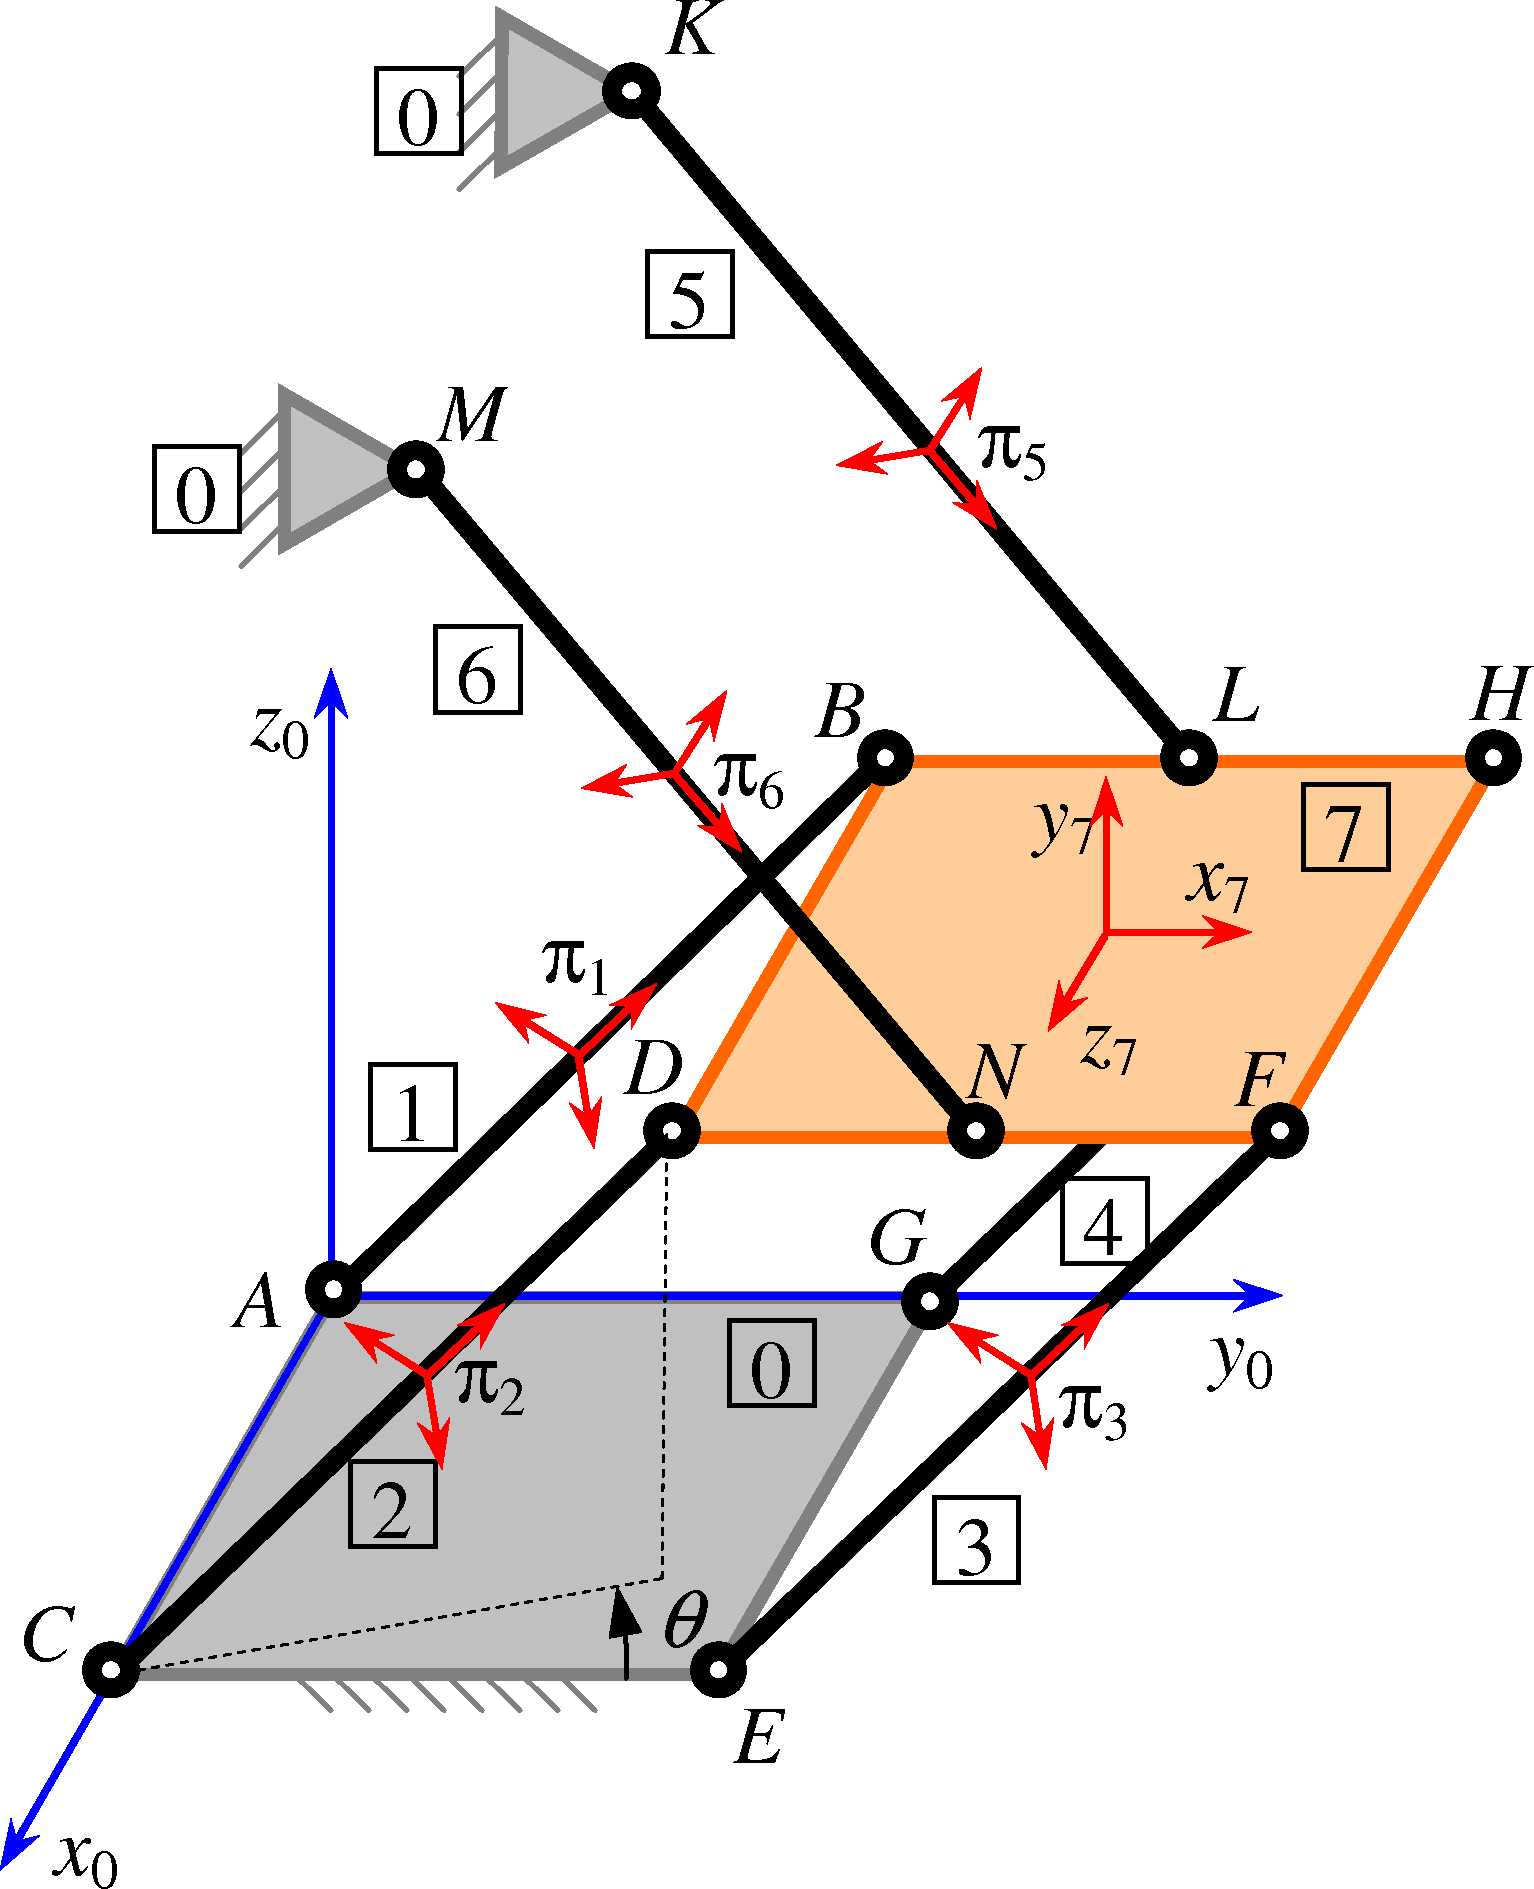
\includegraphics[width=.7\linewidth]{mbs_system.png}
		\captionof{figure}{Multi-body system with 1 DOF}
		\label{fig:mbs}
	\end{minipage}%
	\begin{minipage}{.5\textwidth}
		\centering
		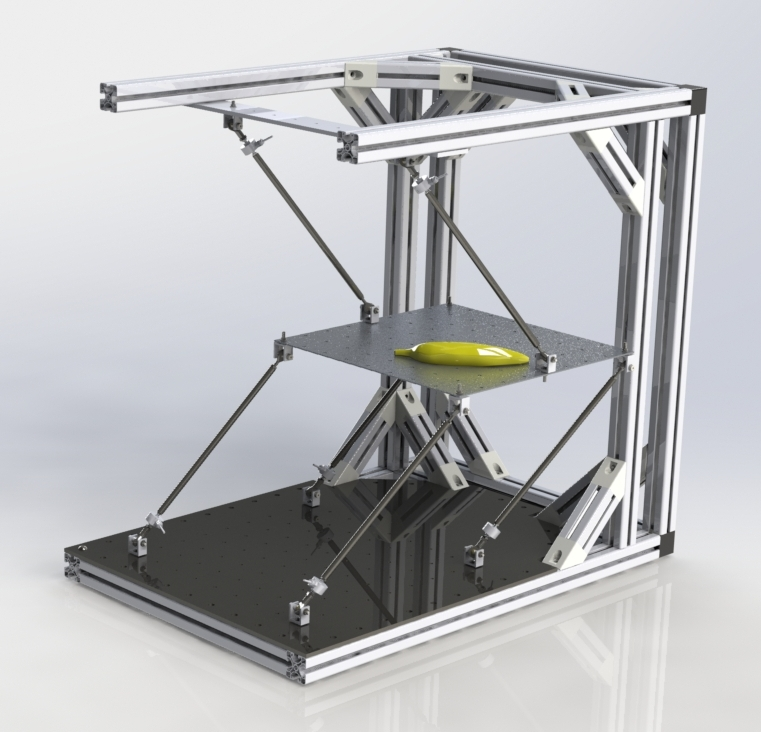
\includegraphics[width=.9\linewidth]{render.jpg}
		\captionof{figure}{Render of the MBS}
		\label{fig:render}
	\end{minipage}
\end{figure}

The scientific significance of this mechanism is revealed in the determination of the reaction forces that occur in rods. The mechanism is statically indeterminate, which makes it even more difficult to analyze and highlights its research value. Further research will require collecting data from the test stand when the platform moves. The state description should contain platform position and orientation as well as readings from the force sensors installed in rods, which will be covered by the system being developed.\\

The mechanism is driven by the FANUC M-10iA serial industrial robot. The robot’s control system tracks the end-effector position. To avoid problems resulting from inaccurate manufacturing and imperfect trajectory execution, the robot is connected to the platform center via a drawbar, so that the imperfections can be compensated by additional -- otherwise not used -- relative motion possibilities. Additionally, such a connection makes the end-effector orientation unimportant. Moreover, the robot position refresh rate is relatively slow but can be successfully used in sensor fusion.\\

The mechanism thus presented is a representative example of the application of the developed measuring system. Due to its properties, conventional methods are hard to apply. The proposed solution is challenging as well, but the procedure that leads to a working system is structured and split into steps. 

\section{Computer simulation}

Before real-life experiments, fundamental aspects of the project were tested in computer simulation. The simulation involves preparing a kinematic model in ADAMS and connecting it with a simplified estimation system in MATLAB Simulink. A ready-to-use model was employed (created earlier as part of the research project). The ADAMS model was extended with a new cylinder-shaped body that represents the robot end-effector. The added part is connected to the moving platform center and was used as the motion source. The simulated position of the end-effector was set as a control variable that constitutes input to the program. The kinematic simulation outputs are the position and orientation of the moving platform, its linear acceleration, and angular velocity expressed in the local coordinate system. These variables will be used to simulate the sensors' readings. An angular velocity is used to simulate a gyroscope, while a linear acceleration is used to simulate an accelerometer. Figure \ref{adams} presents multi-body system modeled in ADAMS software. That prepared model was converted to a Simulink block.

\begin{figure}[!h]
	\centering
	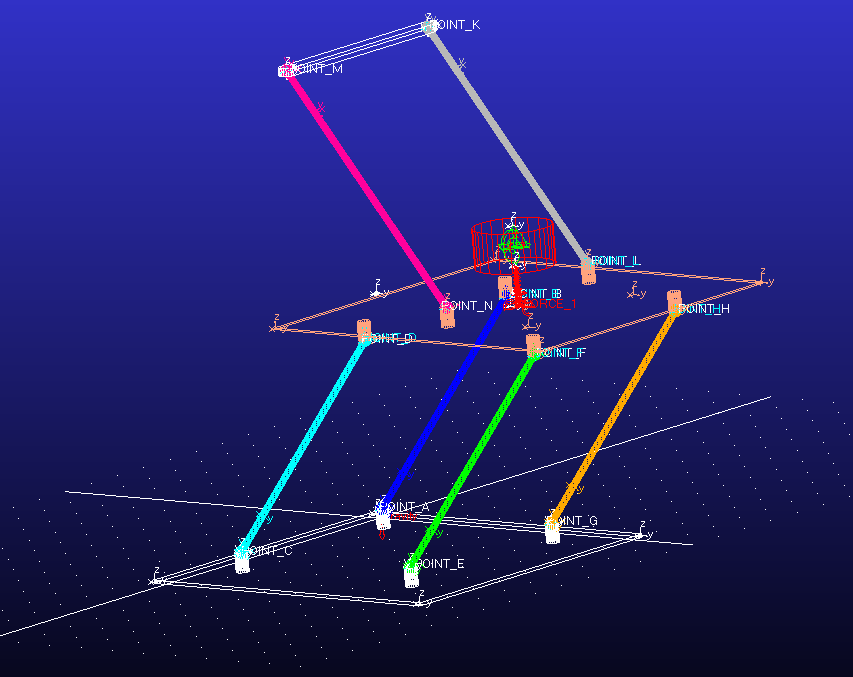
\includegraphics[width=0.6\textwidth]{duw/adams.png}
	\caption{The mechanism modeled in ADAMS software}
	\label{adams}
\end{figure}

Next, to move the mechanism, a trajectory generator was prepared. One of the allowed trajectories is a circular motion in the horizontal plane. In order to check position tracking, the tangential velocity was constantly increased. Equations (\ref{tcp_begin} - \ref{tcp_end}) present the three components of the position of the robot's end-effector as a function of time.

\begin{align}
	x_{TCP} &= x_0 +  R\ cos( t^2 )
	\label{tcp_begin}\\
	y_{TCP} &= y_0  + R\ sin( t^2 )\\
	z_{TCP} &= z_0
	\label{tcp_end}
\end{align}

With the platform that already moves, the following stage is to simulate inertial sensors: an accelerometer and a gyroscope. The sensors are simulated based on ADAMS block outputs. The gyroscope returns an angular velocity, while the accelerometer returns linear velocity with gravitation acceleration added. Figure \ref{acc_sym} presents Simulink blocks that represent an ideal accelerometer.

\begin{figure}[!h]
	\centering
	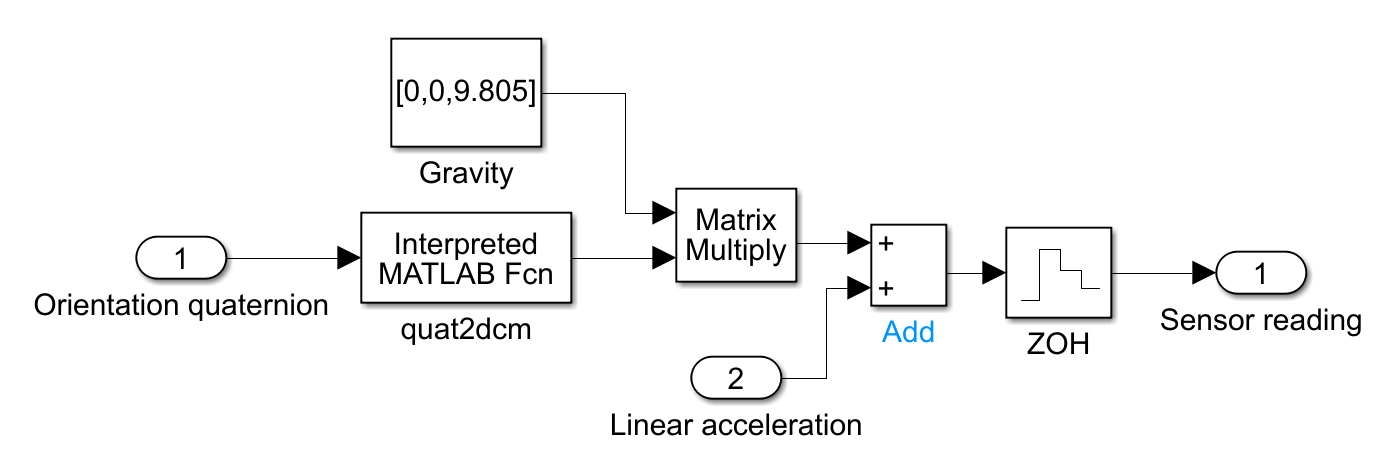
\includegraphics[width=0.75\textwidth]{duw/acc_sim.png}
	\caption{The simulation of an accelerometer}
	\label{acc_sym}
\end{figure}

The output of an ideal sensor simulation is further passed to blocks that represent the sensor error. This simplified simulation limited the sensor error to adding a pink noise and bias. Figure \ref{error_sensor} shows Simulink blocks that represent a sensor error.

\begin{figure}[!h]
	\centering
	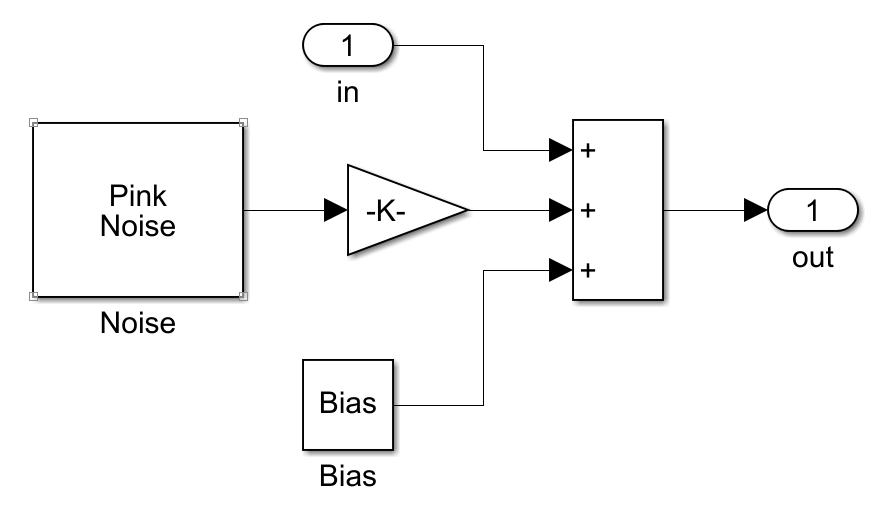
\includegraphics[width=0.6\textwidth]{duw/error.png}
	\caption{The simulation of a sensor error}
	\label{error_sensor}
\end{figure}

The final step was to implement and tune the Kalman Filter with constraints correction. Once again, the MATLAB implementation is a simplified version of the filter described in section \ref{filter_model}. The implemented constraints are given in equation (\ref{simplified_eq} -- \ref{simplified_eq2}). Figure \ref{ekf_sim} presents a realization of the filter in Simulink.

\begin{align}
	x^2 + y^2 - r^2 &= 0
	\label{simplified_eq}\\
	z &= 0
	\label{simplified_eq2}
\end{align}

\begin{figure}[!h]
	\centering
	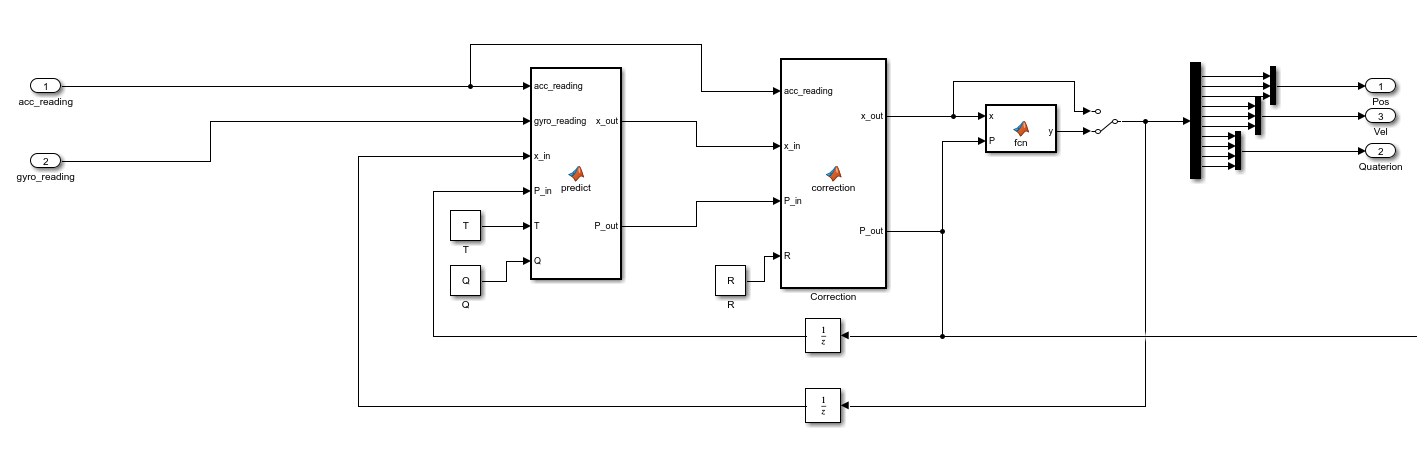
\includegraphics[width=0.9\textwidth]{duw/ekf.png}
	\caption{The Kalman Filter with constraints correction}
	\label{ekf_sim}
\end{figure}
\ \\

That prepared simulation was run multiple times to select the optimal set of parameters. The presented results are the best achieved after the tuning process. First, the filter work was examined without the constraints correction. Figure \ref{no_con} presents the coordinates change as a function of time. The plot includes the robot end-effector position, the moving platform center position, and their estimations. The estimations (magenta, yellow, and blue colors in the plots) drift heavily over simulation time.\\

\begin{figure}[!h]
	\centering
	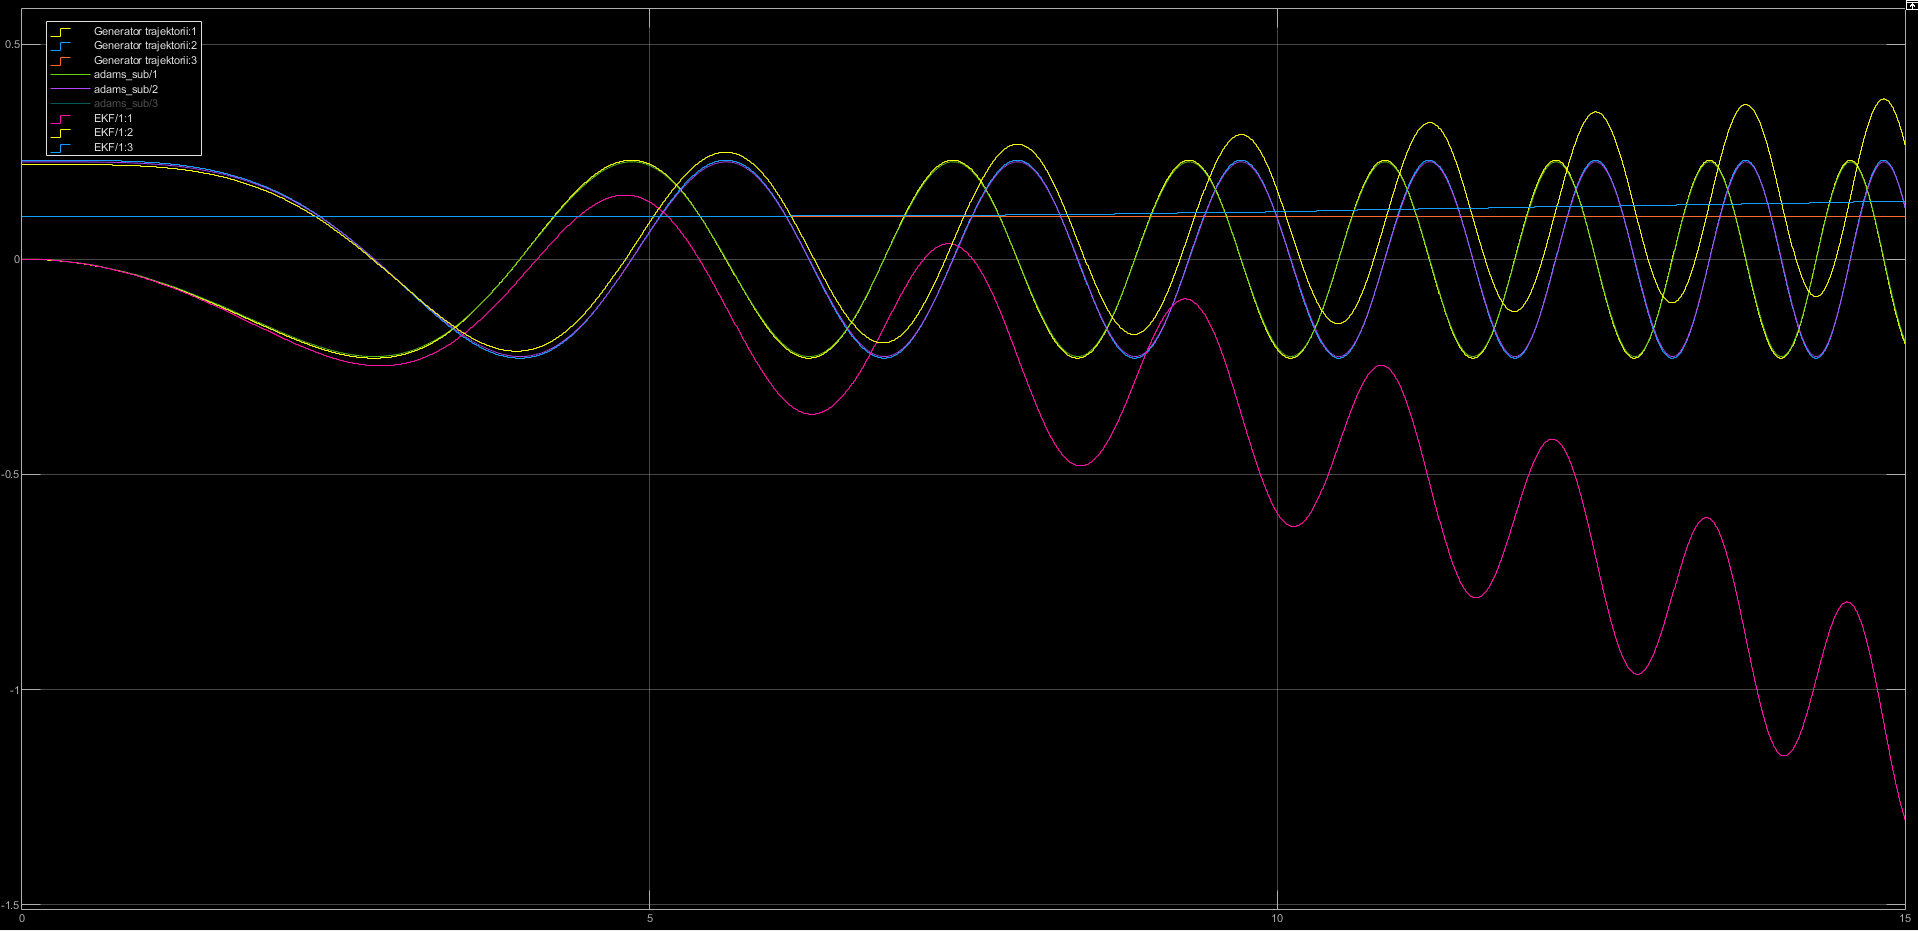
\includegraphics[width=\textwidth]{duw/no_con.png}
	\caption{The result of simulation (without correction)}
	\label{no_con}
\end{figure}

Figure \ref{corr} presents the run of an analogous simulation, however,  with constraints correction turned on. The estimation matches the position for most of the simulation time. During the second revolution, the system lost the tracked value, but the match was quickly restored.

\begin{figure}[!h]
	\centering
	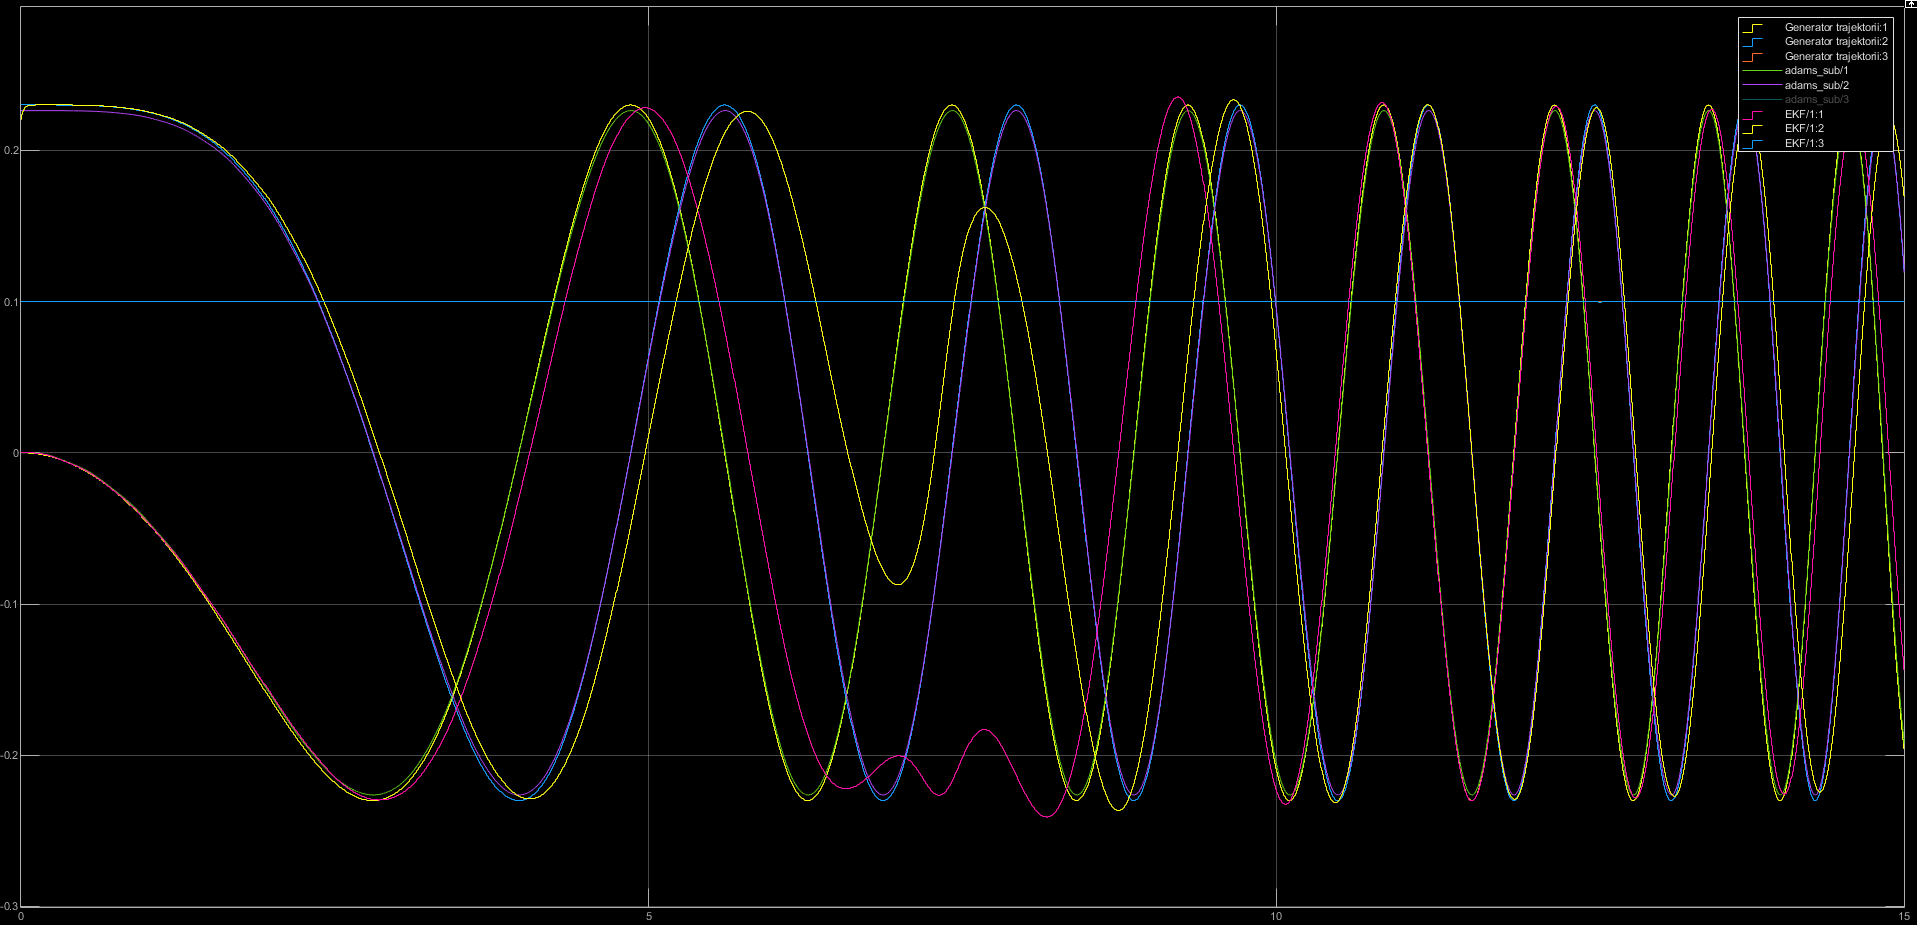
\includegraphics[width=\textwidth]{duw/corr.png}
	\caption{The result of simulation (with correction)}
	\label{corr}
\end{figure}

\newpage
To summarize, the simulation shows a substantial and positive impact of applying correction of constraints. Chronologically, computer simulation was part of the preparations for the realization of this thesis, which energized further work and complete system implementation.